\chapter{研究背景}\label{chap:background}

本章では、プログラムを実行する対象の変化や、その処理領域の変化について述べた後、
これらの変化がもたらす新しいプログラミングの領域について示す。

\section{計算資源としての人}\label{sec:human-as-computational-resouces}

コンピュータのみでは解決が困難な問題を、人間を計算資源として利用することによって解決する考え方は
ヒューマンコンピュテーション\cite{humancomputation}と呼ばれる。
コンピュータは優れた処理能力を有するが、パターン認識能力など人間のほうが得意な処理分野は多く存在する。
これらの分野において人間とコンピュータがお互いの得意な領域で力を発揮することによって、
今までは実現が困難であったような処理でも実現可能となった。

ヒューマンコンピュテーションの例として挙げられるシステムとして、reCAPTCHA\cite{recaptcha}が挙げられる。
reCAPTCHAは、人間かコンピュータを識別するためのテストとして活用されているCAPTCHA\cite{captcha}を応用したものだ。
人間かコンピュータかの識別を行いながら、コンピュータでは識別が困難な文字の認識を人間に実行させるシステムだ。
reCAPTCHAを使うことで、利用者は自分が人間であることを証明しながら、紙の本のデジタル化に貢献している。
文章の校正も人間のほうが得意であったり、内容によっては人間にしかできない作業である。
この文章の校正作業をインターネットを介して他の人間たちに実行させるSoylent\cite{soylent}といったソフトウェアも存在する。
この他にも、多くのヒューマンコンピュテーションの考えを活用したシステムが存在する。

インターネットを介した不特定多数の人間に仕事を依頼する仕組みはクラウドソーシング\cite{riseofcrowdsourcing}と呼ばれる。
必要なときに必要なだけの人材を安価に集めることができ、近年注目を浴びている。
クラウドソーシングにおいてもヒューマンコンピュテーションの考えが反映された事例は多く存在し、
大量の人間を計算資源とした処理が実現されている。

近年ではスマートフォンやタブレットデバイスの普及によって、人間はインターネットを介していつでもあらゆる場所で、
様々なシステムに接続可能となっている。
これは、利用者側にとっては便利にインターネットを介して情報を得られるようになったという側面と共に、
いつでもシステム側から利用者とコミュニケーションが取れるようになったということでもある。
また、気軽に持ち運ぶことができるため、家の中や外出先等、どこでもやりとりができるようになっている。
つまり、いつでもどこでも人間を計算資源として利用する下地が出来つつあるということだ。
計算資源として常時アクセス可能になりつつある人間は、今まで以上に計算資源として利用されると考えられる。

ヒューマンコンピュテーションやクラウドソーシングが広まるにつれ、
人間を優秀な計算資源として捉え活用する事例は増えている。
人間と計算機、どちらが実行するとしても、実現したい処理が可能で結果を得ることが出来れば問題はない。
ある処理を実現する上では、人間もコンピュータも処理を実行するための同じ資源として考えることができる。
プログラムにおける人間と計算機の境界はなくなりつつある。

\section{プログラムの制御領域}\label{sec:are-of-program}

世界中にある様々なコンピュータやデバイスがインターネットに繋がり、プログラムによって制御されるようになってきている。
従来のプログラムは、主に計算機上や画面の中の制御を行うことが多かったが、
近年では、Arduino\footnote{http://www.arduino.cc/}やRaspberryPi\footnote{http://www.raspberrypi.org/}等の登場によって、
誰でも簡単にセンサーやアクチュエータを扱えるようになっている。
実世界から情報を得たり、実世界を制御するためのプログラムは今では誰でも簡単に扱うことができる。
プログラムは実世界を含んだ広い領域の制御のために使われていくと考えられる。

マーク・ワイザーが提唱したユビキタスコンピューティング\cite{weiser1991computer}は、実世界環境にコンピュータを溶けこませ、
ユーザは意識することなくコンピュータによる支援を享受できるという概念だ。
ユビキタスコンピューティングのように、日常生活をコンピュータを用いて支援する仕組みについて研究は多くなされているが、
それらの仕組みの多くはプログラムによって制御されている。
類似の概念としてはInternet of
Things(以下、IoT)\cite{iot}といった考えも提唱されている。
あらゆるモノがインターネットに繋がり、情報をやりとりすることによって様々な恩恵を得ることができるというのが
IoTの基本的な考え方である。
IoTの考えに基づいて様々なモノが繋がれば、プログラムによる実世界の制御はさらに広がるだろう。

また、建築物の構成要素をプログラマブルにする試み\cite{squama}や、
プログラムによってその構成を動的に変化させるモジュールについての研究もなされている。
これらの研究が実用化されていけば、生活空間や物質の制御にもプログラムが利用される。

既にプログラムはあらゆる領域において制御を担っているが、今後は
より多くの領域がプログラムによって制御されるようになると考えられる。

\section{あらゆる処理をプログラムで記述する}\label{ux3042ux3089ux3086ux308bux51e6ux7406ux3092ux30d7ux30edux30b0ux30e9ux30e0ux3067ux8a18ux8ff0ux3059ux308b}

第\ref{#sec:human-as-computational-resouces}節から、プログラムにおいて人間と計算機は
同じ計算資源として振る舞うようになっていくと考えられる。
また、第\ref{#sec:area-of-program}節のように、プログラムが制御を担う領域は今後も広がっていくことが予想される。
プログラムによって実世界の要素を制御することは日常的になっていくと考える。
これらのことから、プログラムは処理する領域を限定することなく、処理を実行する対象も限定することはなくなっていく。
つまり、プログラムは人間と計算機の双方を用いて実世界・電子世界の双方を処理することのできる環境が出来上がるということである。

このような環境が実現すれば、実世界におけるタスクを人間に処理させるといったことが可能となり、
今までは実現できなかったような処理をプログラムとして記述できるようになる。
例えば、料理をするプログラムといったものが可能だ。
料理レシピは調理する上で必要となる処理を記述するものであり、プログラムと似ている。
人間はこのレシピを見て、実行すべき処理を読み取り、その内容に従って処理を実行する。
料理レシピの一部をプログラムとして記述するならば、図\ref{fig:background_cooking}のようになる。

\begin{figure}[htbp]
  \begin{center}
  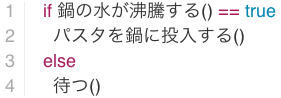
\includegraphics[width=.4\linewidth,bb=0 0 281 98]{images/background_cooking.js.png}
  \end{center}
  \caption{料理レシピの一部をプログラム風に記述する}
  \label{fig:background_cooking}
\end{figure}

また、仕事のマニュアルなども同様である。
その時々で行うべき業務はマニュアルなどによって定義されており、人間はマニュアルを見たり、覚えておくことによって
処理を実行する。
例えば、小売店の店員の仕事は図\ref{fig:background_retail}のようなプログラムとして記述可能である。

\begin{figure}[htbp]
  \begin{center}
  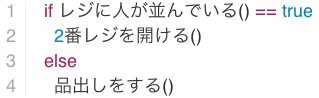
\includegraphics[width=.4\linewidth,bb=0 0 319 98]{images/background_retail.js.png}
  \end{center}
  \caption{小売店の店員の挙動の一部をプログラム風に記述する}
  \label{fig:background_retail}
\end{figure}

レシピやマニュアルといったように、人間が実行すべき処理を記述してある手順書は多く存在する。
これは、ただ実行する対象が人間なだけであって、プログラムと同類のものであると言える。
人間にとっての処理もコンピュータにとっての処理も、ほぼ同じ記法で記述することが可能だ。
今まで実世界で人間が行っていたようなタスクは、プログラムに変換可能である。

上記のようなタスクをプログラムとして記述し実行することによって、処理に応じて
人間と計算機を切り替えて実行させ、分業させることが可能となる。
計算機が得意なことは計算機が、人が得意なことは人が実行するようにすれば、より効率的であったり、
確実性の高い処理が実現する。
可能な限り計算機に処理を実行させることで、人間の負担を減らすことも可能だ。

そもそも、人間と計算機では得意な分野や実現可能な処理が異なる。
人間は柔軟な思考能力や身体を所有することから、パターン認識や感性判断の必要な処理、
実世界から情報を取得したり、干渉することが得意である。
また、意思決定も人間が実行すべき処理だ。
計算機は高速な演算能力を有することから、計算や記憶、正確なセンシングなどを担うべきである。

実世界のタスク等の記述も含めた、人間とコンピュータの処理を融合させたプログラムを記述することが出来れば、
コンピュータによる支援を受けたより効率的なタスク実行などが可能となり、有用である言える。
このような、人間とコンピュータはお互いの得意な領域において処理を実行し、両者が密接に関わりあうことで、
より知的で効率的な処理を実現するという考えは、Lickliderが人間とコンピュータの共生\cite{man-computer-symbiosis}という
概念として提唱しており、人間とコンピュータの共生が望まれている。

しかし、現状では人間とコンピュータの処理を融合させたプログラムを実行するような環境は十分に整っていない。
人間とコンピュータをプログラム上において同じような記法で扱える仕組みはクラウドソーシング分野での利用に限られている。
想定する利用シーンは知的活動に限られており、実世界でのタスクを処理するようなことには向いていない。
「料理をする」といったプログラムは、インターネットを介した他人に実行してもらっても無意味である。
また、自分の日常的な活動をプログラムで記述したいという時でも、自分自身を実行対象にすることができない。
家庭内でのタスクをプログラムしたい場合であれば、家族に実行対象を限定したい。
これらの問題から、クラウドソーシングを利用した手法は実世界のタスクを処理するためのプログラムを実行する用途には向かない。

そこで、本研究では、人間と計算機の処理を融合させることのできるプログラミング環境を提案する。
このプログラミング環境は以下のような特徴を持つ

\begin{itemize}
\itemsep1pt\parskip0pt\parsep0pt
\item
  人間と計算機への指示を類似の記法で実現
\item
  実行者を具体的に指定可能
\item
  実世界のタスクを処理することを考慮した実装
\end{itemize}

本研究で提案するプログラミング環境によって、新しいプログラミングの可能性を追求する。

\section{まとめ}\label{ux307eux3068ux3081}

本章では、プログラムの現状について示し、人間とコンピュータが対等な処理実行のリソースであるということを示した。
また、プログラムが実行対象を選ばない汎用的な処理記述フォーマットであることを示し、あらゆる処理を記述するためのプログラミング環境の実現に向けた
状況を考察した。
